\documentclass[border=10pt]{standalone} 
\usepackage{tikz}

\usetikzlibrary{calc}
\usetikzlibrary{arrows}
\usetikzlibrary{shadows}
\usetikzlibrary{patterns}
\usetikzlibrary{positioning}
\usetikzlibrary{shapes}
\usetikzlibrary{3d}
%\usetikzlibrary{automata}
\usetikzlibrary{fit}

\tikzset{block/.style={draw, text centered, fill=gray!10,drop shadow}}
\tikzset{connect/.style={draw, line width=1 pt}}

\begin{document}


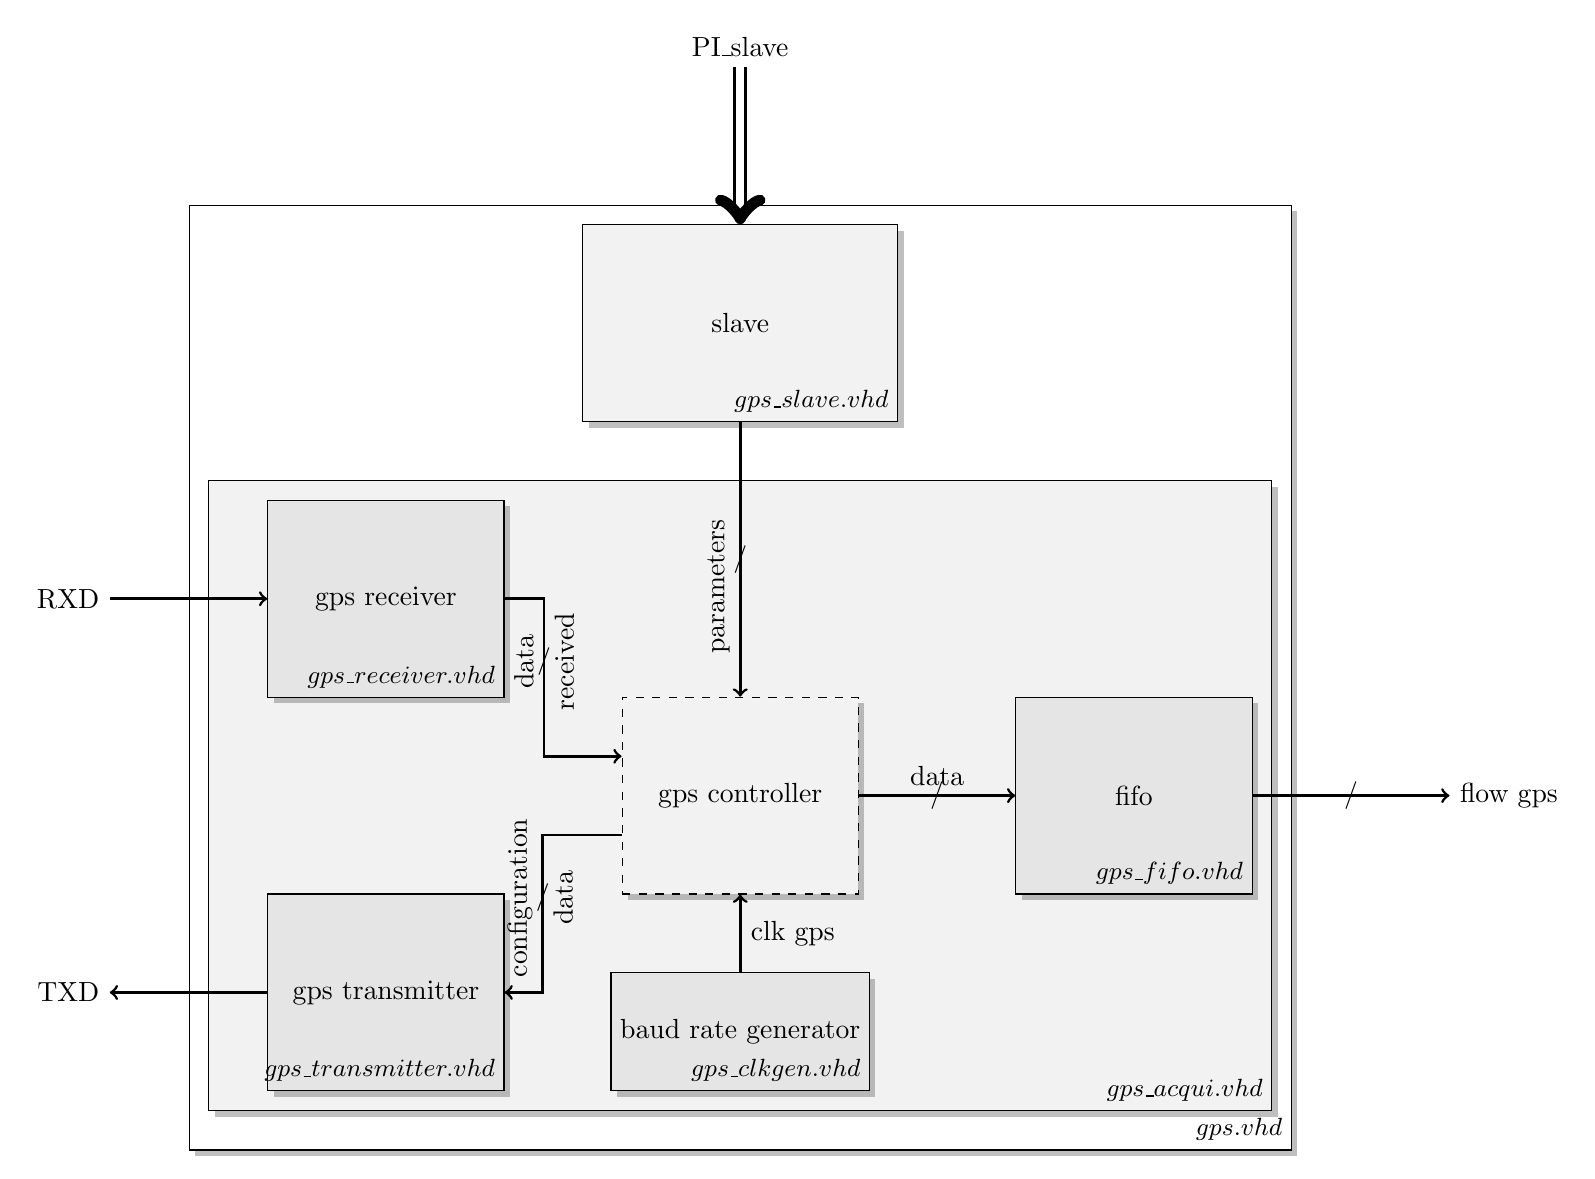
\begin{tikzpicture}



\node[block,minimum height=12cm,minimum width=14cm, fill=white] (bloc) {top\_GPS};
\draw (bloc.south east) node[above left]{\small $gps.vhd$} ;

%sub block
\node[block,rectangle,minimum height=8cm,minimum width=13.5cm, fill=gray!10] (gps) at([yshift=-1.5cm]bloc) { };
\draw (gps.south east) node[above left]{\small $gps\_acqui.vhd$} ;

%receiver and transmitter
\node[block,rectangle,minimum height=2.5cm,minimum width=3cm,fill=gray!20] (receiver) at([yshift=2.5cm,xshift=-4.5cm]gps) {gps receiver};
\draw (receiver.south east) node[above left]{\small $gps\_receiver.vhd$} ;
\node[block,rectangle,minimum height=2.5cm,minimum width=3cm,fill=gray!20] (transmitter) at([yshift=-2.5cm,xshift=-4.5cm]gps) {gps transmitter};
\draw (transmitter.south east) node[above left]{\small $gps\_transmitter.vhd$} ;

%Fifo gps
\node[block,rectangle,minimum height=2.5cm,minimum width=3cm,fill=gray!20] (fifo) at([xshift=5cm]gps) {fifo};
\draw (fifo.south east) node[above left]{\small $gps\_fifo.vhd$} ;

%clk gen
\node[block,rectangle,minimum height=1.5cm,minimum width=3cm,fill=gray!20] (gen) at([yshift=-3cm]gps) {baud rate generator};
\draw (gen.south east) node[above left]{\small $gps\_clkgen.vhd$} ;

%controller
\node[block,rectangle,minimum height=2.5cm,minimum width=3cm,fill=gray!10,dashed] (controller) at(gps) {gps controller};


%external ports
\path[connect,<-] (receiver.west) -- ++ (-2cm,0) node[left]{RXD};
\path[connect,->] (transmitter.west) -- ++ (-2cm,0) node[left]{TXD};


%flows out
\path[connect,->] (fifo.east) -- node{/} ++(2.5cm,0) node[right]{flow gps};


%Slave and connections
\node[block,rectangle,minimum height=2.5cm,minimum width=4cm,fill=gray!10] (slave) at([yshift=4.5cm]bloc) {slave};
\draw (slave.south east) node[above left]{\small $gps\_slave.vhd$} ;
\path[connect,<-][double distance = 3pt] (slave.north)  -- ++(0,2cm) node[above]{PI\_slave};

%internal connections
\path[connect,->] (slave.south)  -- node{/} node[above,pos=0.6,rotate=90]{parameters} (controller.north)  ;
\path[connect,->] (gen.north)  -- node[right]{clk gps} (controller.south)  ;
\path[connect,->] (receiver.east)  -|  ([xshift=0.5cm]receiver.east) |- node[pos=0.2]{/} node[above,pos=0.20,rotate=90]{data} node[below,pos=0.20,rotate=90]{received} ([yshift=0.5cm]controller.west)  ;
\path[connect,->] ([yshift=-0.5cm]controller.west)  -|  ([xshift=-1cm,yshift=-0.5cm]controller.west) |- node[above,pos=0.20,rotate=90]{configuration} node[pos=0.2]{/} node[below,pos=0.20,rotate=90]{data} (transmitter.east)  ;
\path[connect,->] (controller.east) -- node[above]{data}node{/} (fifo.west)  ;



\end{tikzpicture}


\end{document}